\begin{enumerate}[label=\thechapter.\arabic*,ref=\thechapter.\theenumi]
\item A sinusoidal message signal having root mean square value of 4V and frequency of 1 kHz fed to a phase modulator with phase deviation constant 2 rad/volt. If the carrier signal is $c\brak{t} = 2\cos \brak{2\pi 10^6 t}$, the maximum instantaneous frequency of the phase modulated signal (rounded off to one decimal place) is \rule{1cm}{0.05mm} Hz. \hfill(GATE 2021 EC)\\
\solution\\
\iffalse
\documentclass[journal,12pt,twocolumn]{IEEEtran}
\usepackage{amsmath,amssymb,amsfonts,amsthm}
\usepackage{txfonts}
\usepackage{tkz-euclide}
\usepackage[margin=0.25in]{geometry}
\usepackage{pgfplots}
\usepackage{listings}
\usepackage{gvv}
\usepackage[latin1]{inputenc}
\usepackage{adjustbox}
\usepackage{array}
\usepackage{tabularx}
\usepackage{enumitem}
\usepackage{pgf}
\usepackage{lmodern}
\usepackage{circuitikz}
\usepackage{tikz}
\usepackage{graphicx}
\pgfplotsset{width=10cm,compat=1.18}

\begin{document}
\bibliographystyle{IEEEtran}

\vspace{3cm}

\title{}
\author{EE23BTECH11054 -  Sai Krishna Shanigarapu$^{*}$
}
\maketitle
\newpage
\bigskip

\section*{Gate EC 2021}
49. \hspace{2pt} A sinusoidal message signal having root mean square value of 4V and frequency of 1 kHz fed to a phase modulator with phase deviation constant 2 rad/volt. If the carrier signal is $c\brak{t} = 2\cos \brak{2\pi 10^6 t}$, the maximum instantaneous frequency of the phase modulated signal (rounded off to one decimal place) is \rule{1cm}{0.05mm} Hz. \hfill(GATE 2021 EC)\\
\solution\\
\fi
\begin{table}[ht]
    \centering
    \setlength{\arrayrulewidth}{0.3mm}
\setlength{\tabcolsep}{20pt}
\renewcommand{\arraystretch}{1.5}


\begin{tabular}{|c|c|c|}
\hline
Parameter & Description & Value\\
\hline
$f_m$ & Message signal frequency & 1 kHz\\
\hline
$c\brak{t}$ & Carrier signal & $2\cos \brak{2\pi 10^6 t}$\\
\hline
$k_p$ & Phase sensitivity factor & 2 rad $V^{-1}$\\
\hline
$m\brak{t}$ &  message signal & $A_m\sin{2\pi f_m t}$\\
\hline
$f_c$ & Carrier signal frequency & 1 kHz\\
\hline
$A_c$ & Amplitude of carrier signal & 2 \\
\hline
$A_m$ & Amplitude of message signal & \\
\hline
\end{tabular}
    \caption{Input Parameters}
    \label{tab:tab1_gate_2021_ec_49}
\end{table}

\begin{table}[ht]
    \centering
    \setlength{\arrayrulewidth}{0.3mm}
\setlength{\tabcolsep}{20pt}
\renewcommand{\arraystretch}{1.6}


\begin{tabular}{|c|c|c|}
\hline
Parameter & Description & Formula\\
\hline
$m\brak{t}_{rms}$ & rms value of $m\brak{t}$ & $\frac{A_m}{\sqrt{2}}$\\
\hline
$s\brak{t}$ & Phase modulation & $A_c\sin \sbrak{2\pi f_c t + \theta _i\brak{t}}$\\
\hline
$\theta _i\brak{t}$ & phase & $k_p\, m\brak{t}$\\
\hline
\end{tabular}

    \caption{Formulae}
    \label{tab:tab2_gate_2021_ec_49}
\end{table}

Phase Modulation Signal Proof:\\
let $e_m$ and $e_c$ be message and carrier signals, $2\pi f_m$ and $2\pi f_c$ be radial frequencies and $A_m$ and $A_c$ be their amplitudes respectively. Then,
\begin{align}
	e_m &= A_m\cos \brak{2\pi f_m t}\\
	e_c &= A_c \sin \brak{2\pi f_c t} \label{eq:test1_21_ec49}
\end{align}
On rewriting the equation \ref{eq:test1_21_ec49}
\begin{align}
	e &= E_c\sin \brak{\theta}\\
	\theta &= 2\pi f_c t + k_p e_m\\
	&= 2\pi f_c t + k_pE_m\cos \brak{2\pi f_m t}\\
	m_p &= k_p E_m\\
	\theta &= 2\pi f_c t + m_p\cos \brak{2\pi f_m t}\\
	\implies s\brak{t} &= E_c\sin \brak{2\pi f_c t + \underbrace{m_p\cos \brak{2\pi f_m t}}_\text{$\theta_i \brak{t}$}} \label{eq:test2_21_ec49}
\end{align}

\begin{align}
    m\brak{t}_{rms} &= 4V \label{eq:eq1_gate_2021_ec_49} \\
    A_m &= 4\sqrt{2} \label{eq:eq2_gate_2021_ec_49}
\end{align}
From Table \ref{tab:tab1_gate_2021_ec_49}, eq (\ref{eq:eq1_gate_2021_ec_49}) and eq (\ref{eq:eq2_gate_2021_ec_49})
\begin{align}
     m\brak{t} &= 4\sqrt{2}\sin \brak{2 \pi 10^3 t}\\
\end{align}

\begin{figure}[ht]
    \centering
    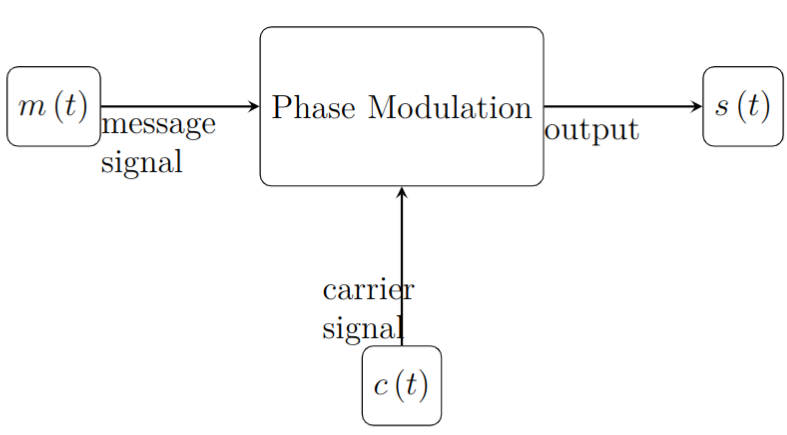
\includegraphics[width=\columnwidth]{2021/EC/49/figs/fig2.png}
    \caption{Block diagram of phase modulation}
    \label{fig:fig1_gate_2021_ec_49}  
\end{figure}
From Table \ref{tab:tab1_gate_2021_ec_49}, \ref{tab:tab2_gate_2021_ec_49} and using eq (\ref{eq:test2_21_ec49}) instantaneous frequency is given as,
\begin{align}
    f_i\brak{t} &= f_c + \frac{1}{2\pi}\, \frac{d}{dt}\theta_i\brak{t}\\
    &= f_c + \frac{1}{2\pi}\, \frac{d}{dt}\sbrak{k_p m\brak{t}}\\
    &= f_c + \frac{1}{2\pi}\, \frac{d}{dt}\brak{4\sqrt{2}\sin \brak{2 \pi 10^3 t}}\\
    &= f_c + \frac{2}{2\pi}\, 4\sqrt{2}\, \brak{2\pi 10^3}\, \brak{\cos \brak{2 \pi 10^3 t}}\\
    &= 1000 + 8\sqrt{2} \text{ x } 10^3 \cos \brak{2\pi 10^3 t}
\end{align}
Thus,
\begin{align}
    \implies f_{i_{max}} &= 1011313.7 \, Hz
\end{align}

\begin{figure}[ht]
    \centering
        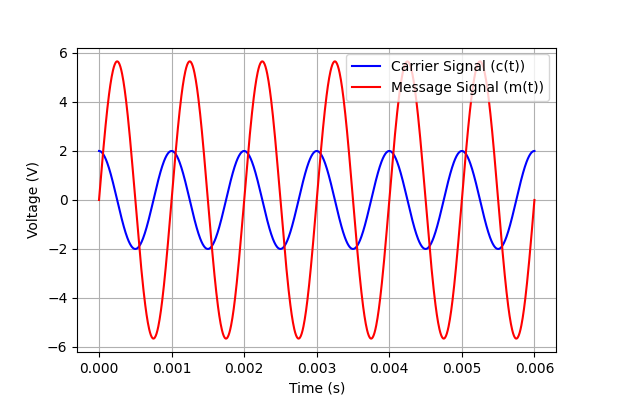
\includegraphics[width=\columnwidth]{2021/EC/49/figs/Figure_1.png}
    \caption{plot of $m\brak{t}$ and $c\brak{t}$}
\end{figure}

%\end{document}

\pagebreak
\item Two discrete-time linear time-invarient systems with impulse responses $h_1[n]=\delta[n-1]+\delta[n+1]$ and $h_2[n]=\delta[n]+\delta[n-1]$ are connected in cascade, where $\delta[n]$ is the Kronecker delta. The impulse response of the cascaded system is   \\
\begin{enumerate}[label=(\alph*)]
    \item $\delta[n-2]+\delta[n+1]$
    \item $\delta[n-1]\delta[n]+\delta[n+1]\delta[n-1]$
    \item $\delta[n-2]+\delta[n-1]+\delta[n]+\delta[n+1]$
    \item $\delta[n]\delta[n-1]+\delta[n-2]\delta[n+1]$
\end{enumerate} \hfill(GATE 2021 EE)\\
\solution
\iffalse
\let\negmedspace\undefined
\let\negthickspace\undefined
\documentclass[journal,12pt,twocolumn]{IEEEtran}
\usepackage{cite}
\usepackage{amsmath,amssymb,amsfonts,amsthm}
\usepackage{algorithmic}
\usepackage{graphicx}
\usepackage{textcomp}
\usepackage{xcolor}
\usepackage{pgfplots}
\usepackage{txfonts}
\usepackage{listings}
\usepackage{enumitem}
\usepackage{mathtools}
\usepackage{gensymb}
\usepackage{comment}
\usepackage[breaklinks=true]{hyperref}
\usepackage{tkz-euclide} 
\usepackage{listings}
\usepackage{gvv}                                        
\def\inputGnumericTable{}                                 
\usepackage[latin1]{inputenc}                                
\usepackage{color}                                            
\usepackage{array}                                            
\usepackage{longtable}                                       
\usepackage{calc}                                             
\usepackage{multirow}                                         
\usepackage{hhline}                                           
\usepackage{ifthen}                                           
\usepackage{lscape}

\newtheorem{theorem}{Theorem}[section]
\newtheorem{problem}{Problem}
\newtheorem{proposition}{Proposition}[section]
\newtheorem{lemma}{Lemma}[section]
\newtheorem{corollary}[theorem]{Corollary}
\newtheorem{example}{Example}[section]
\newtheorem{definition}[problem]{Definition}
\newcommand{\BEQA}{\begin{eqnarray}}
\newcommand{\EEQA}{\end{eqnarray}}
\newcommand{\define}{\stackrel{\triangle}{=}}
\theoremstyle{remark}
\newtheorem{rem}{Remark}
\begin{document}
\parindent 0px
\bibliographystyle{IEEEtran}
\title{GATE: EE - 7.2021}
\author{EE22BTECH11219 - Rada Sai Sujan$^{}$% <-this % stops a space
}
\maketitle
\newpage
\bigskip
\section*{Question}
Two discrete-time linear time-invarient systems with impulse responses $h_1[n]=\delta[n-1]+\delta[n+1]$ and $h_2[n]=\delta[n]+\delta[n-1]$ are connected in cascade, where $\delta[n]$ is the Kronecker delta. The impulse response of the cascaded system is   \\
\begin{enumerate}[label=(\alph*)]
    \item $\delta[n-2]+\delta[n+1]$
    \item $\delta[n-1]\delta[n]+\delta[n+1]\delta[n-1]$
    \item $\delta[n-2]+\delta[n-1]+\delta[n]+\delta[n+1]$
    \item $\delta[n]\delta[n-1]+\delta[n-2]\delta[n+1]$
\end{enumerate} \hfill(GATE 2021 EE)\\
\solution
\fi

\begin{figure}[ht]
    \centering
    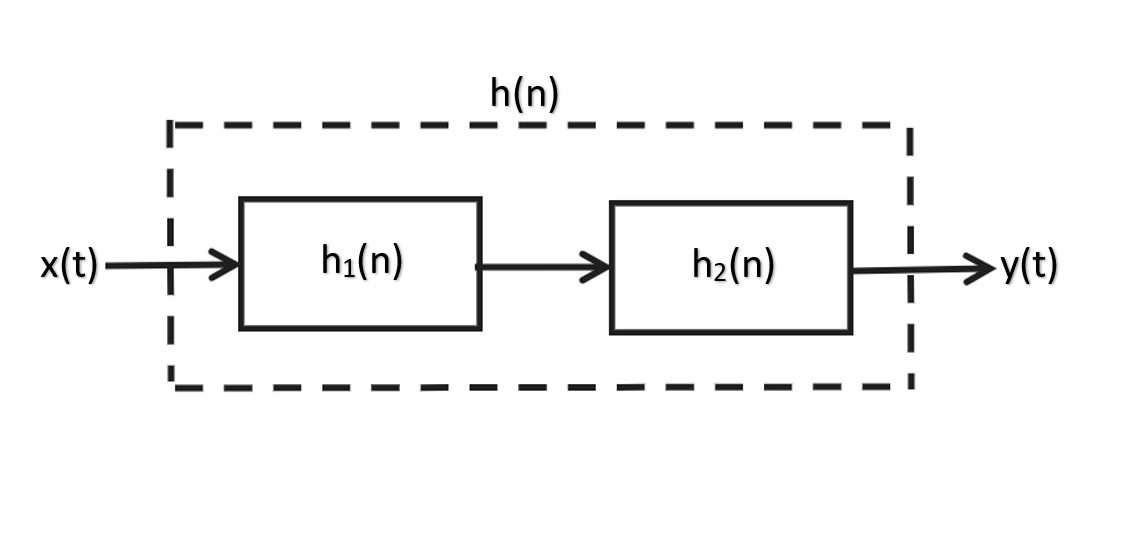
\includegraphics[width=\columnwidth]{2021/EE/7/figs/fig2.png}
    \caption{Block Diagram}
    \label{fig:g2022ee7.2}
\end{figure}  
From the $Z$-transformation pairs,
\begin{align}
    \delta[n] &\overset{\mathcal{Z}}{ \longleftrightarrow} 1  \label{eqn:g22ee7.1}  \\
    x\brak{n-k} &\overset{\mathcal{Z}}{ \longleftrightarrow} z^{-k}X\brak{z} \label{eqn:g22ee7.2}   \\
    x_1\brak{n}\ast x_2\brak{n} &\overset{\mathcal{Z}}{ \longleftrightarrow} X_1\brak{z}X_2\brak{z} \label{eqn:g22ee7.3}
\end{align}
If $h_1\brak{n}$ and $h_2\brak{n}$ are cascade connected then the resultant impulse can be given by:
\begin{align}
    h\brak{n}&=h_1\brak{n}\ast h_2\brak{n}    \\
    \implies H\brak{z}&=H_1\brak{z}H_2\brak{z}    \\
    H\brak{z}&=\brak{z^{-1}+z}\brak{1+z^{-1}}   \\
    &=\brak{z^{-1}+z^{-2}+z+1}, \quad \abs{z}\neq 0
\end{align}
Using the $Z$-transformation pairs to find the the inverse $Z$-transform,
\begin{align}
    h\brak{n}&=\delta[n-2]+\delta[n-1]+\delta[n]+\delta[n+1]
\end{align}
\begin{figure}[ht]
    \centering
    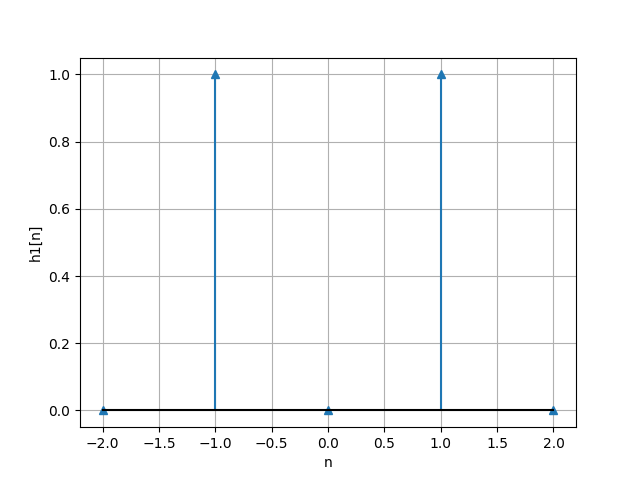
\includegraphics[width=\columnwidth]{2021/EE/7/figs/fig3.png}
    \caption{$h_1\brak{n}$ $vs$ $n$ graph}
    \label{fig:g2022ee7.3}
\end{figure}     
\begin{figure}[ht]
    \centering
    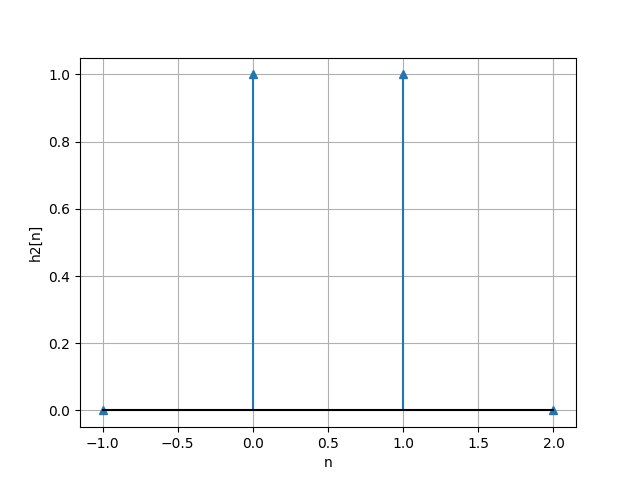
\includegraphics[width=\columnwidth]{2021/EE/7/figs/fig4.png}
    \caption{$h_2\brak{n}$ $vs$ $n$ graph}
    \label{fig:g2022ee7.4}
\end{figure}     
\begin{figure}[ht]
    \centering
    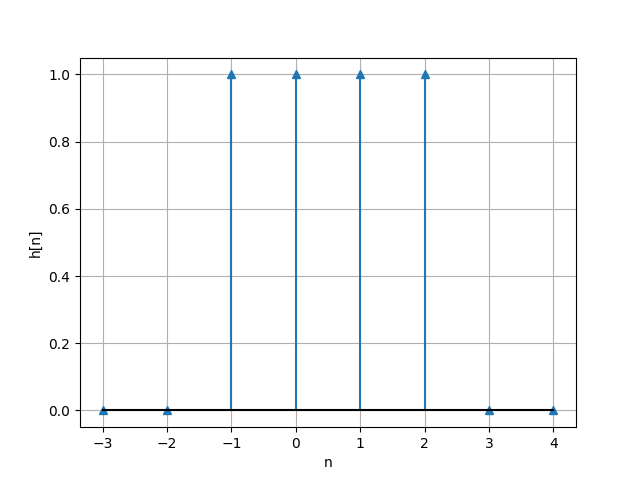
\includegraphics[width=\columnwidth]{2021/EE/7/figs/fig1.png}
    \caption{$h\brak{n}$ $vs$ $n$ graph}
    \label{fig:g2022ee7.1}
\end{figure}

\pagebreak
\item Consider a superheterodyne receiver tuned to 600 kHz. If the local oscillator feeds a 1000 kHz signal to the mixer, the image frequency (in integer) is \underline{\hspace{1cm}} kHz.
\hfill(GATE EC 2021)\\
\solution
\iffalse
\documentclass{article}
\usepackage{tikz}
\usetikzlibrary{positioning, arrows.meta, shapes.geometric, shapes.multipart}
\usepackage{amsmath}

\begin{document}

Consider a superheterodyne receiver tuned to 600 kHz. If the local oscillator feeds a 1000 kHz signal to the mixer, the image frequency (in integer) is \underline{\hspace{1cm}} kHz.
\hfill(GATE EC 2021)\\

\textbf{Solution:}
\fi
\begin{table}[h]
    \centering
    \begin{tabular}{|c|c|c|}
        \hline
        \textbf{Parameter} & \textbf{Symbol} & \textbf{Value} \\
        \hline
        Receiver Frequency & \(f_r\) & 600 kHz \\
        \hline
        Local Oscillator Frequency & \(f_l\) & 1000 kHz \\
        \hline
        Image Frequency & \(f_i\) & \underline{\hspace{2cm}} kHz \\
        \hline
    \end{tabular}
    \caption{Given Parameters with Symbols}
\end{table}

Let \(f_x\) be the intermediate frequency given by \(|f_l - f_r|\).
\begin{align}
    f_x &= |1000-600| = 400 \, \text{kHz}
\end{align}
\begin{figure}[htb]
 \centering
\begin{tikzpicture}
    \draw (0,0) -- (6,0);
    \draw[thick,->] (1,0) -- node[below=4mm] {$f_r$} (1,1);
    \draw[thick,->] (3,0) -- node[below=14mm] {$f_l$} (3,3);
    \draw[thick,->] (5,0) --  node[below=4mm] {$f_i$}(5,1);
    \draw[<->] (1.25,0.5) --node[above] {$f_x$}(2.75,0.5);
    \draw[<->] (3.25,0.5) --node[above] {$f_x$}(4.75,0.5);
\end{tikzpicture}
 \caption{Diagram}
    \label{fig:reflection}
\end{figure}



From the above diagram, we can observe that:
\begin{align}
    f_i &= f_r+2(f_x) = 600+2(400)=1400 \, \text{kHz}
\end{align}
Therefore the Image frequency is \textbf{1400 kHz}
\begin{figure}
    \centering
    \begin{tikzpicture}[
        block/.style={draw, rectangle, minimum height=1.5cm, text width=3cm, align=center},
        arrow/.style={->, >=Stealth},
        node distance=2cm
    ]

    % Nodes
    \node[block] (mixer) {Mixer};
    \node[block, below=of mixer] (if) {Intermediate\\Frequency\\($f_x = 400$ kHz)};
    \node[block, below=of if] (lo) {Local Oscillator\\($f_r = 1000$ kHz)};
    \node[block, below=of lo] (rf) {RF Signal\\($f_l = 600$ kHz)};
    \node[block, right=of if, xshift=2cm] (image) {Image Frequency\\($f_i = 1400$ kHz)};

    % Arrows
    \draw[arrow] (rf) -- (lo);
    \draw[arrow] (lo) -- (if);
    \draw[arrow] (mixer) -- (if);
    \draw[arrow] (if) -- (image);

    \end{tikzpicture}
    \caption{Superheterodyne Receiver Block Diagram}
\end{figure}


%\end{document}


\pagebreak
\item In the block diagram shown below, an infinite tap FIR filter with transfer function $H\brak{z}=\frac{Y\brak{z}}{X\brak{z}}$ is realized. If $H\brak{z}=\frac{1}{1-0.5z^{-1}}$.\\the value of $\alpha$ is
\begin{figure}[h]
    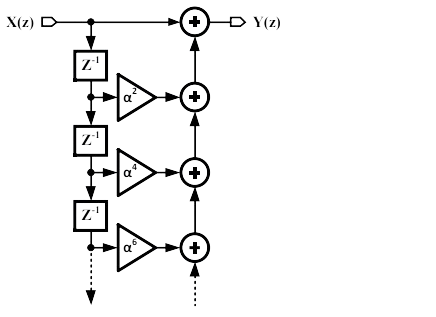
\includegraphics[width=1\columnwidth]{2021/BM/31/figs/questionfig.png}
    \label{fig:question31bm}
\end{figure} \hfill(GATE 2021 BM)\\
\solution
 \iffalse
\let\negmedspace\undefined
\let\negthickspace\undefined
\documentclass[journal,12pt,twocolumn]{IEEEtran}
\usepackage{cite}
\usepackage{amsmath,amssymb,amsfonts,amsthm}
\usepackage{algorithmic}
\usepackage{graphicx}
\usepackage{textcomp}
\usepackage{xcolor}
\usepackage{txfonts}
\usepackage{listings}
\usepackage{enumitem}
\usepackage{mathtools}
\usepackage{gensymb}
\usepackage{comment}
\usepackage{tikz}
\usepackage[breaklinks=true,hidelinks]{hyperref}
\usepackage{tkz-euclide} 
\usepackage{listings}
\usepackage{gvv}
\def\inputGnumericTable{}
\usepackage[latin1]{inputenc}                              
\usepackage{color} 
\usepackage{array}                                            
\usepackage{longtable}                                       
\usepackage{calc}                                             
\usepackage{multirow}                                         
\usepackage{hhline}                                           
\usepackage{ifthen}                                           
\usepackage{lscape}

\newtheorem{theorem}{Theorem}[section]
\newtheorem{problem}{Problem}
\newtheorem{proposition}{Proposition}[section]
\newtheorem{lemma}{Lemma}[section]
\newtheorem{corollary}[theorem]{Corollary}
\newtheorem{example}{Example}[section]
\newtheorem{definition}[problem]{Definition}
\newcommand{\BEQA}{\begin{eqnarray}}
\newcommand{\EEQA}{\end{eqnarray}}
\newcommand{\define}{\stackrel{\triangle}{=}}
\theoremstyle{remark}
\newtheorem{rem}{Remark}
\begin{document}

\bibliographystyle{IEEEtran}
\vspace{3cm}

\title{GATE 2021 BM Q-31}
\author{EE23BTECH11207 -KAILASH.C$^{*}$% <-this % stops a space
}
\maketitle
\newpage
\bigskip

\renewcommand{\thefigure}{\theenumi}
\renewcommand{\thetable}{\theenumi}
In the block diagram shown below, an infinite tap FIR filter with transfer function $H\brak{z}=\frac{Y\brak{z}}{X\brak{z}}$ is realized. If $H\brak{z}=\frac{1}{1-0.5z^{-1}}$.\\the value of $\alpha$ is
\begin{figure}[h]
    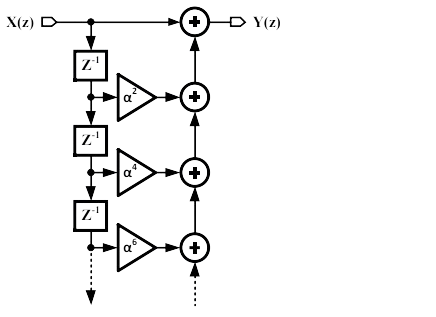
\includegraphics[width=1\columnwidth]{2021/BM/31/figs/questionfig.png}
    \label{fig:question31bm}
\end{figure} \hfill(GATE 2021 BM)\\
\solution
\fi
\begin{table}[h]
\begin{tabular}{|l|l|l|}
\hline
\textbf{Parameter} & \textbf{Definition}\\ \hline
$H\brak{z} & $\frac{1}{1-0.5z^{-1}}$ \\ \hline
\end{tabular}
\caption{Parameter Table}
\label{tab:gate.bm.31.2021}
\end{table}
\\
From diagram we have:
\begin{align}
    Y\brak{z}&=X\brak{z}\brak{\sum_{n=0}^{\infty}\brak{z^{-1}\alpha^{2}}^n}\label{eq:311_bm}
\end{align}
Dividing by $X\brak{z}$ in both sides:
\begin{align}
    \frac{Y\brak{z}}{X\brak{z}}&=\sum_{n=0}^{\infty}\brak{z^{-1}\alpha^{2}}^n\label{eq:312_bm}\\
    \implies H\brak{z}&=\sum_{n=0}^{\infty}\brak{z^{-1}\alpha^{2}}^n\label{eq:313_bm}\\
    \frac{1}{1-0.5z^{-1}}&=\sum_{n=0}^{\infty}\brak{z^{-1}\alpha^{2}}^n\label{eq:314_bm}\\
\frac{1}{1-0.5z^{-1}}&=\frac{1}{1-z^{-1}\alpha^{2}}\label{eq:315_bm}\\
\implies \alpha&=\frac{1}{\sqrt{2}}\label{eq:316_bm}
\end{align}

\pagebreak
\end{enumerate}
